% Paper Fig. 2 (pipeline), extracted from the NeurIPS 2026 camera-ready source for the docs.
\documentclass[border=4pt]{standalone}
\usepackage[T1]{fontenc}
\usepackage{tikz}
\usetikzlibrary{arrows.meta, positioning, fit}
\begin{document}
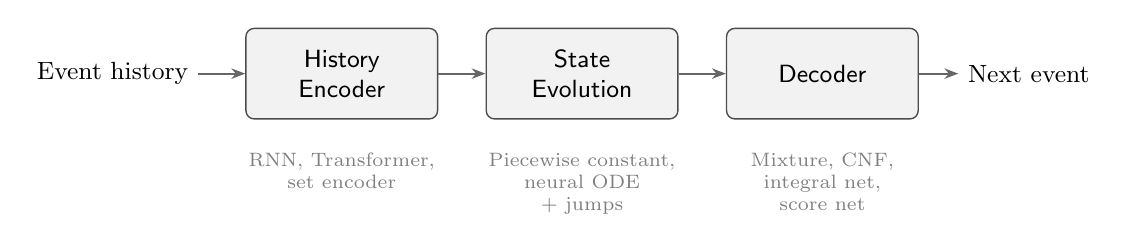
\begin{tikzpicture}[
    node distance=0.6cm,
    box/.style={
        rectangle, rounded corners=3pt, draw=black!70, fill=black!5,
        minimum height=1.15cm, minimum width=2.3cm,
        text centered, font=\small\sffamily, text width=2.2cm,
        line width=0.5pt
    },
    io/.style={
        font=\small
    },
    arr/.style={
        -{Stealth[length=5pt]}, thick, black!60
    },
    note/.style={
        font=\scriptsize, text=black!50, text width=2.4cm, text centered
    }
]

% Input
\node[io] (input) {Event history};

% Three boxes
\node[box, right=of input] (enc) {History\\Encoder};
\node[box, right=of enc]   (evo) {State\\Evolution};
\node[box, right=of evo]   (dec) {Decoder};

% Output
\node[io, right=0.5cm of dec] (output) {Next event};

% Arrows
\draw[arr] (input) -- (enc);
\draw[arr] (enc) -- (evo);
\draw[arr] (evo) -- (dec);
\draw[arr] (dec) -- (output);

% Bottom annotations
\node[note, below=0.3cm of enc]
    {RNN, Transformer,\\set encoder};
\node[note, below=0.3cm of evo]
    {Piecewise constant,\\neural ODE + jumps};
\node[note, below=0.3cm of dec]
    {Mixture, CNF,\\integral net, score net};

\end{tikzpicture}
\end{document}
